

\tikzset{every picture/.style={line width=0.75pt}} %set default line width to 0.75pt        

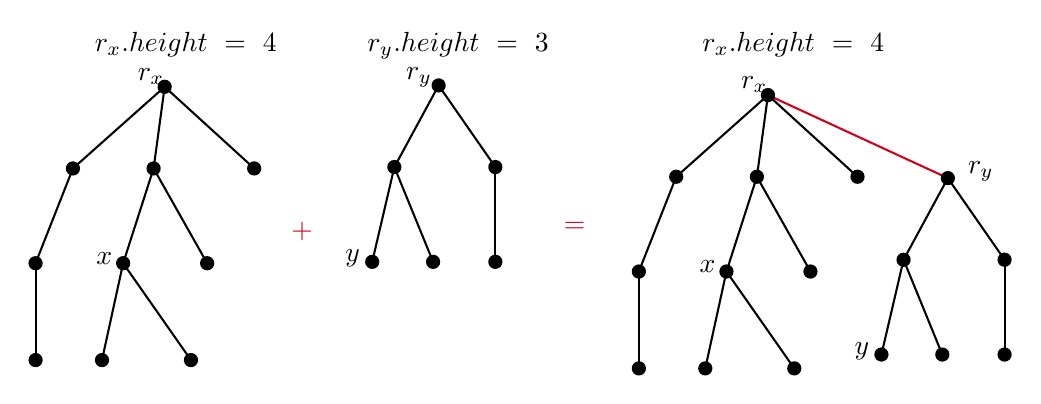
\begin{tikzpicture}[x=0.5pt,y=0.5pt,yscale=-1,xscale=1]
%uncomment if require: \path (0,281); %set diagram left start at 0, and has height of 281

%Flowchart: Connector [id:dp9897896441945839] 
\draw  [fill={rgb, 255:red, 0; green, 0; blue, 0 }  ,fill opacity=1 ] (105.59,53.9) .. controls (106.45,51.65) and (108.99,50.52) .. (111.24,51.39) .. controls (113.5,52.26) and (114.62,54.79) .. (113.75,57.05) .. controls (112.88,59.3) and (110.35,60.43) .. (108.1,59.56) .. controls (105.84,58.69) and (104.72,56.16) .. (105.59,53.9) -- cycle ;
%Flowchart: Connector [id:dp8075110738416615] 
\draw  [fill={rgb, 255:red, 0; green, 0; blue, 0 }  ,fill opacity=1 ] (39.29,112.9) .. controls (40.16,110.65) and (42.69,109.52) .. (44.95,110.39) .. controls (47.2,111.26) and (48.33,113.79) .. (47.46,116.05) .. controls (46.59,118.3) and (44.06,119.43) .. (41.8,118.56) .. controls (39.55,117.69) and (38.42,115.16) .. (39.29,112.9) -- cycle ;
%Straight Lines [id:da9902964456425614] 
\draw [color={rgb, 255:red, 208; green, 2; blue, 27 }  ,draw opacity=1 ]   (545.67,61.48) -- (675.67,121.48) ;
%Straight Lines [id:da5172177882024809] 
\draw    (43.37,114.48) -- (109.67,55.48) ;
%Flowchart: Connector [id:dp11019606064742127] 
\draw  [fill={rgb, 255:red, 0; green, 0; blue, 0 }  ,fill opacity=1 ] (97.59,112.9) .. controls (98.45,110.65) and (100.99,109.52) .. (103.24,110.39) .. controls (105.5,111.26) and (106.62,113.79) .. (105.75,116.05) .. controls (104.88,118.3) and (102.35,119.43) .. (100.1,118.56) .. controls (97.84,117.69) and (96.72,115.16) .. (97.59,112.9) -- cycle ;
%Flowchart: Connector [id:dp28900689737394614] 
\draw  [fill={rgb, 255:red, 0; green, 0; blue, 0 }  ,fill opacity=1 ] (170.29,112.9) .. controls (171.16,110.65) and (173.69,109.52) .. (175.95,110.39) .. controls (178.2,111.26) and (179.33,113.79) .. (178.46,116.05) .. controls (177.59,118.3) and (175.06,119.43) .. (172.8,118.56) .. controls (170.55,117.69) and (169.42,115.16) .. (170.29,112.9) -- cycle ;
%Flowchart: Connector [id:dp8349300680889286] 
\draw  [fill={rgb, 255:red, 0; green, 0; blue, 0 }  ,fill opacity=1 ] (75.59,181.4) .. controls (76.45,179.15) and (78.99,178.02) .. (81.24,178.89) .. controls (83.5,179.76) and (84.62,182.29) .. (83.75,184.55) .. controls (82.88,186.8) and (80.35,187.93) .. (78.1,187.06) .. controls (75.84,186.19) and (74.72,183.66) .. (75.59,181.4) -- cycle ;
%Flowchart: Connector [id:dp5271991889149706] 
\draw  [fill={rgb, 255:red, 0; green, 0; blue, 0 }  ,fill opacity=1 ] (12.29,181.4) .. controls (13.16,179.15) and (15.69,178.02) .. (17.95,178.89) .. controls (20.2,179.76) and (21.33,182.29) .. (20.46,184.55) .. controls (19.59,186.8) and (17.06,187.93) .. (14.8,187.06) .. controls (12.55,186.19) and (11.42,183.66) .. (12.29,181.4) -- cycle ;
%Flowchart: Connector [id:dp4031153203734361] 
\draw  [fill={rgb, 255:red, 0; green, 0; blue, 0 }  ,fill opacity=1 ] (12.29,251.4) .. controls (13.16,249.15) and (15.69,248.02) .. (17.95,248.89) .. controls (20.2,249.76) and (21.33,252.29) .. (20.46,254.55) .. controls (19.59,256.8) and (17.06,257.93) .. (14.8,257.06) .. controls (12.55,256.19) and (11.42,253.66) .. (12.29,251.4) -- cycle ;
%Flowchart: Connector [id:dp0008363872359773428] 
\draw  [fill={rgb, 255:red, 0; green, 0; blue, 0 }  ,fill opacity=1 ] (136.29,181.4) .. controls (137.16,179.15) and (139.69,178.02) .. (141.95,178.89) .. controls (144.2,179.76) and (145.33,182.29) .. (144.46,184.55) .. controls (143.59,186.8) and (141.06,187.93) .. (138.8,187.06) .. controls (136.55,186.19) and (135.42,183.66) .. (136.29,181.4) -- cycle ;
%Flowchart: Connector [id:dp7716868638159723] 
\draw  [fill={rgb, 255:red, 0; green, 0; blue, 0 }  ,fill opacity=1 ] (124.59,251.4) .. controls (125.45,249.15) and (127.99,248.02) .. (130.24,248.89) .. controls (132.5,249.76) and (133.62,252.29) .. (132.75,254.55) .. controls (131.88,256.8) and (129.35,257.93) .. (127.1,257.06) .. controls (124.84,256.19) and (123.72,253.66) .. (124.59,251.4) -- cycle ;
%Flowchart: Connector [id:dp8451689968178246] 
\draw  [fill={rgb, 255:red, 0; green, 0; blue, 0 }  ,fill opacity=1 ] (60.29,251.4) .. controls (61.16,249.15) and (63.69,248.02) .. (65.95,248.89) .. controls (68.2,249.76) and (69.33,252.29) .. (68.46,254.55) .. controls (67.59,256.8) and (65.06,257.93) .. (62.8,257.06) .. controls (60.55,256.19) and (59.42,253.66) .. (60.29,251.4) -- cycle ;
%Flowchart: Connector [id:dp032017927511610256] 
\draw  [fill={rgb, 255:red, 0; green, 0; blue, 0 }  ,fill opacity=1 ] (303.59,52.9) .. controls (304.45,50.65) and (306.99,49.52) .. (309.24,50.39) .. controls (311.5,51.26) and (312.62,53.79) .. (311.75,56.05) .. controls (310.88,58.3) and (308.35,59.43) .. (306.1,58.56) .. controls (303.84,57.69) and (302.72,55.16) .. (303.59,52.9) -- cycle ;
%Flowchart: Connector [id:dp7753230180353938] 
\draw  [fill={rgb, 255:red, 0; green, 0; blue, 0 }  ,fill opacity=1 ] (271.59,111.9) .. controls (272.45,109.65) and (274.99,108.52) .. (277.24,109.39) .. controls (279.5,110.26) and (280.62,112.79) .. (279.75,115.05) .. controls (278.88,117.3) and (276.35,118.43) .. (274.1,117.56) .. controls (271.84,116.69) and (270.72,114.16) .. (271.59,111.9) -- cycle ;
%Flowchart: Connector [id:dp7480294214835582] 
\draw  [fill={rgb, 255:red, 0; green, 0; blue, 0 }  ,fill opacity=1 ] (255.59,180.4) .. controls (256.45,178.15) and (258.99,177.02) .. (261.24,177.89) .. controls (263.5,178.76) and (264.62,181.29) .. (263.75,183.55) .. controls (262.88,185.8) and (260.35,186.93) .. (258.1,186.06) .. controls (255.84,185.19) and (254.72,182.66) .. (255.59,180.4) -- cycle ;
%Flowchart: Connector [id:dp4873571062167924] 
\draw  [fill={rgb, 255:red, 0; green, 0; blue, 0 }  ,fill opacity=1 ] (344.59,111.9) .. controls (345.45,109.65) and (347.99,108.52) .. (350.24,109.39) .. controls (352.5,110.26) and (353.62,112.79) .. (352.75,115.05) .. controls (351.88,117.3) and (349.35,118.43) .. (347.1,117.56) .. controls (344.84,116.69) and (343.72,114.16) .. (344.59,111.9) -- cycle ;
%Flowchart: Connector [id:dp4230951468351575] 
\draw  [fill={rgb, 255:red, 0; green, 0; blue, 0 }  ,fill opacity=1 ] (344.59,180.4) .. controls (345.45,178.15) and (347.99,177.02) .. (350.24,177.89) .. controls (352.5,178.76) and (353.62,181.29) .. (352.75,183.55) .. controls (351.88,185.8) and (349.35,186.93) .. (347.1,186.06) .. controls (344.84,185.19) and (343.72,182.66) .. (344.59,180.4) -- cycle ;
%Flowchart: Connector [id:dp02723705167497803] 
\draw  [fill={rgb, 255:red, 0; green, 0; blue, 0 }  ,fill opacity=1 ] (299.59,180.4) .. controls (300.45,178.15) and (302.99,177.02) .. (305.24,177.89) .. controls (307.5,178.76) and (308.62,181.29) .. (307.75,183.55) .. controls (306.88,185.8) and (304.35,186.93) .. (302.1,186.06) .. controls (299.84,185.19) and (298.72,182.66) .. (299.59,180.4) -- cycle ;
%Straight Lines [id:da8485530944868279] 
\draw    (16.37,182.98) -- (43.37,114.48) ;
%Straight Lines [id:da936425631795308] 
\draw    (79.67,182.98) -- (101.67,114.48) ;
%Straight Lines [id:da3467674009082027] 
\draw    (101.67,114.48) -- (109.67,55.48) ;
%Straight Lines [id:da2710068544626746] 
\draw    (174.37,114.48) -- (109.67,55.48) ;
%Straight Lines [id:da18129286507358067] 
\draw    (140.37,182.98) -- (101.67,114.48) ;
%Straight Lines [id:da44262512432909795] 
\draw    (16.37,252.98) -- (16.37,182.98) ;
%Straight Lines [id:da31047061197895953] 
\draw    (64.37,252.98) -- (79.67,182.98) ;
%Straight Lines [id:da7822071001867994] 
\draw    (128.67,252.98) -- (79.67,182.98) ;
%Straight Lines [id:da8032171189474756] 
\draw    (275.67,113.48) -- (307.67,54.48) ;
%Straight Lines [id:da8169278171705383] 
\draw    (259.67,181.98) -- (275.67,113.48) ;
%Straight Lines [id:da4835943452382059] 
\draw    (303.67,181.98) -- (275.67,113.48) ;
%Straight Lines [id:da6486207879374191] 
\draw    (348.67,113.48) -- (307.67,54.48) ;
%Straight Lines [id:da5877844887696961] 
\draw    (348.67,181.98) -- (348.67,113.48) ;
%Flowchart: Connector [id:dp20762635887871939] 
\draw  [fill={rgb, 255:red, 0; green, 0; blue, 0 }  ,fill opacity=1 ] (541.59,59.9) .. controls (542.45,57.65) and (544.99,56.52) .. (547.24,57.39) .. controls (549.5,58.26) and (550.62,60.79) .. (549.75,63.05) .. controls (548.88,65.3) and (546.35,66.43) .. (544.1,65.56) .. controls (541.84,64.69) and (540.72,62.16) .. (541.59,59.9) -- cycle ;
%Flowchart: Connector [id:dp5761285936520872] 
\draw  [fill={rgb, 255:red, 0; green, 0; blue, 0 }  ,fill opacity=1 ] (475.29,118.9) .. controls (476.16,116.65) and (478.69,115.52) .. (480.95,116.39) .. controls (483.2,117.26) and (484.33,119.79) .. (483.46,122.05) .. controls (482.59,124.3) and (480.06,125.43) .. (477.8,124.56) .. controls (475.55,123.69) and (474.42,121.16) .. (475.29,118.9) -- cycle ;
%Straight Lines [id:da47437536489118703] 
\draw    (479.37,120.48) -- (545.67,61.48) ;
%Flowchart: Connector [id:dp9973180956089771] 
\draw  [fill={rgb, 255:red, 0; green, 0; blue, 0 }  ,fill opacity=1 ] (533.59,118.9) .. controls (534.45,116.65) and (536.99,115.52) .. (539.24,116.39) .. controls (541.5,117.26) and (542.62,119.79) .. (541.75,122.05) .. controls (540.88,124.3) and (538.35,125.43) .. (536.1,124.56) .. controls (533.84,123.69) and (532.72,121.16) .. (533.59,118.9) -- cycle ;
%Flowchart: Connector [id:dp7887397130476378] 
\draw  [fill={rgb, 255:red, 0; green, 0; blue, 0 }  ,fill opacity=1 ] (606.29,118.9) .. controls (607.16,116.65) and (609.69,115.52) .. (611.95,116.39) .. controls (614.2,117.26) and (615.33,119.79) .. (614.46,122.05) .. controls (613.59,124.3) and (611.06,125.43) .. (608.8,124.56) .. controls (606.55,123.69) and (605.42,121.16) .. (606.29,118.9) -- cycle ;
%Flowchart: Connector [id:dp9416096601548867] 
\draw  [fill={rgb, 255:red, 0; green, 0; blue, 0 }  ,fill opacity=1 ] (511.59,187.4) .. controls (512.45,185.15) and (514.99,184.02) .. (517.24,184.89) .. controls (519.5,185.76) and (520.62,188.29) .. (519.75,190.55) .. controls (518.88,192.8) and (516.35,193.93) .. (514.1,193.06) .. controls (511.84,192.19) and (510.72,189.66) .. (511.59,187.4) -- cycle ;
%Flowchart: Connector [id:dp3290524933044451] 
\draw  [fill={rgb, 255:red, 0; green, 0; blue, 0 }  ,fill opacity=1 ] (448.29,187.4) .. controls (449.16,185.15) and (451.69,184.02) .. (453.95,184.89) .. controls (456.2,185.76) and (457.33,188.29) .. (456.46,190.55) .. controls (455.59,192.8) and (453.06,193.93) .. (450.8,193.06) .. controls (448.55,192.19) and (447.42,189.66) .. (448.29,187.4) -- cycle ;
%Flowchart: Connector [id:dp0667118668486314] 
\draw  [fill={rgb, 255:red, 0; green, 0; blue, 0 }  ,fill opacity=1 ] (448.29,257.4) .. controls (449.16,255.15) and (451.69,254.02) .. (453.95,254.89) .. controls (456.2,255.76) and (457.33,258.29) .. (456.46,260.55) .. controls (455.59,262.8) and (453.06,263.93) .. (450.8,263.06) .. controls (448.55,262.19) and (447.42,259.66) .. (448.29,257.4) -- cycle ;
%Flowchart: Connector [id:dp9716822322363012] 
\draw  [fill={rgb, 255:red, 0; green, 0; blue, 0 }  ,fill opacity=1 ] (572.29,187.4) .. controls (573.16,185.15) and (575.69,184.02) .. (577.95,184.89) .. controls (580.2,185.76) and (581.33,188.29) .. (580.46,190.55) .. controls (579.59,192.8) and (577.06,193.93) .. (574.8,193.06) .. controls (572.55,192.19) and (571.42,189.66) .. (572.29,187.4) -- cycle ;
%Flowchart: Connector [id:dp48717164529435164] 
\draw  [fill={rgb, 255:red, 0; green, 0; blue, 0 }  ,fill opacity=1 ] (560.59,257.4) .. controls (561.45,255.15) and (563.99,254.02) .. (566.24,254.89) .. controls (568.5,255.76) and (569.62,258.29) .. (568.75,260.55) .. controls (567.88,262.8) and (565.35,263.93) .. (563.1,263.06) .. controls (560.84,262.19) and (559.72,259.66) .. (560.59,257.4) -- cycle ;
%Flowchart: Connector [id:dp18114130792127026] 
\draw  [fill={rgb, 255:red, 0; green, 0; blue, 0 }  ,fill opacity=1 ] (496.29,257.4) .. controls (497.16,255.15) and (499.69,254.02) .. (501.95,254.89) .. controls (504.2,255.76) and (505.33,258.29) .. (504.46,260.55) .. controls (503.59,262.8) and (501.06,263.93) .. (498.8,263.06) .. controls (496.55,262.19) and (495.42,259.66) .. (496.29,257.4) -- cycle ;
%Flowchart: Connector [id:dp7518877314640476] 
\draw  [fill={rgb, 255:red, 0; green, 0; blue, 0 }  ,fill opacity=1 ] (671.59,119.9) .. controls (672.45,117.65) and (674.99,116.52) .. (677.24,117.39) .. controls (679.5,118.26) and (680.62,120.79) .. (679.75,123.05) .. controls (678.88,125.3) and (676.35,126.43) .. (674.1,125.56) .. controls (671.84,124.69) and (670.72,122.16) .. (671.59,119.9) -- cycle ;
%Flowchart: Connector [id:dp599431917297237] 
\draw  [fill={rgb, 255:red, 0; green, 0; blue, 0 }  ,fill opacity=1 ] (639.59,178.9) .. controls (640.45,176.65) and (642.99,175.52) .. (645.24,176.39) .. controls (647.5,177.26) and (648.62,179.79) .. (647.75,182.05) .. controls (646.88,184.3) and (644.35,185.43) .. (642.1,184.56) .. controls (639.84,183.69) and (638.72,181.16) .. (639.59,178.9) -- cycle ;
%Flowchart: Connector [id:dp16343923312842312] 
\draw  [fill={rgb, 255:red, 0; green, 0; blue, 0 }  ,fill opacity=1 ] (623.59,247.4) .. controls (624.45,245.15) and (626.99,244.02) .. (629.24,244.89) .. controls (631.5,245.76) and (632.62,248.29) .. (631.75,250.55) .. controls (630.88,252.8) and (628.35,253.93) .. (626.1,253.06) .. controls (623.84,252.19) and (622.72,249.66) .. (623.59,247.4) -- cycle ;
%Flowchart: Connector [id:dp6848727750904735] 
\draw  [fill={rgb, 255:red, 0; green, 0; blue, 0 }  ,fill opacity=1 ] (712.59,178.9) .. controls (713.45,176.65) and (715.99,175.52) .. (718.24,176.39) .. controls (720.5,177.26) and (721.62,179.79) .. (720.75,182.05) .. controls (719.88,184.3) and (717.35,185.43) .. (715.1,184.56) .. controls (712.84,183.69) and (711.72,181.16) .. (712.59,178.9) -- cycle ;
%Flowchart: Connector [id:dp8120790196669959] 
\draw  [fill={rgb, 255:red, 0; green, 0; blue, 0 }  ,fill opacity=1 ] (712.59,247.4) .. controls (713.45,245.15) and (715.99,244.02) .. (718.24,244.89) .. controls (720.5,245.76) and (721.62,248.29) .. (720.75,250.55) .. controls (719.88,252.8) and (717.35,253.93) .. (715.1,253.06) .. controls (712.84,252.19) and (711.72,249.66) .. (712.59,247.4) -- cycle ;
%Flowchart: Connector [id:dp3775740881604551] 
\draw  [fill={rgb, 255:red, 0; green, 0; blue, 0 }  ,fill opacity=1 ] (667.59,247.4) .. controls (668.45,245.15) and (670.99,244.02) .. (673.24,244.89) .. controls (675.5,245.76) and (676.62,248.29) .. (675.75,250.55) .. controls (674.88,252.8) and (672.35,253.93) .. (670.1,253.06) .. controls (667.84,252.19) and (666.72,249.66) .. (667.59,247.4) -- cycle ;
%Straight Lines [id:da001803532705640376] 
\draw    (452.37,188.98) -- (479.37,120.48) ;
%Straight Lines [id:da647457490609615] 
\draw    (515.67,188.98) -- (537.67,120.48) ;
%Straight Lines [id:da4980390431112198] 
\draw    (537.67,120.48) -- (545.67,61.48) ;
%Straight Lines [id:da6214247879507085] 
\draw    (610.37,120.48) -- (545.67,61.48) ;
%Straight Lines [id:da10843359313978695] 
\draw    (576.37,188.98) -- (537.67,120.48) ;
%Straight Lines [id:da41275684445149585] 
\draw    (452.37,258.98) -- (452.37,188.98) ;
%Straight Lines [id:da1532167517032782] 
\draw    (500.37,258.98) -- (515.67,188.98) ;
%Straight Lines [id:da9072254965197083] 
\draw    (564.67,258.98) -- (515.67,188.98) ;
%Straight Lines [id:da49132027020689406] 
\draw    (643.67,180.48) -- (675.67,121.48) ;
%Straight Lines [id:da5453594011228895] 
\draw    (627.67,248.98) -- (643.67,180.48) ;
%Straight Lines [id:da9542661262103859] 
\draw    (671.67,248.98) -- (643.67,180.48) ;
%Straight Lines [id:da6774988416466069] 
\draw    (716.67,180.48) -- (675.67,121.48) ;
%Straight Lines [id:da1951736113047675] 
\draw    (716.67,248.98) -- (716.67,180.48) ;

% Text Node
\draw (58,173) node [anchor=north west][inner sep=0.75pt]   [align=left] {$\displaystyle x$};
% Text Node
\draw (88,40) node [anchor=north west][inner sep=0.75pt]   [align=left] {$\displaystyle r_{x}$};
% Text Node
\draw (238,171) node [anchor=north west][inner sep=0.75pt]   [align=left] {$\displaystyle y$};
% Text Node
\draw (282,39) node [anchor=north west][inner sep=0.75pt]   [align=left] {$\displaystyle r_{y}$};
% Text Node
\draw (494,179) node [anchor=north west][inner sep=0.75pt]   [align=left] {$\displaystyle x$};
% Text Node
\draw (524,46) node [anchor=north west][inner sep=0.75pt]   [align=left] {$\displaystyle r_{x}$};
% Text Node
\draw (606,238) node [anchor=north west][inner sep=0.75pt]   [align=left] {$\displaystyle y$};
% Text Node
\draw (688,107) node [anchor=north west][inner sep=0.75pt]   [align=left] {$\displaystyle r_{y}$};
% Text Node
\draw (199,151) node [anchor=north west][inner sep=0.75pt]   [align=left] {$\displaystyle \textcolor[rgb]{0.82,0.01,0.11}{+}$};
% Text Node
\draw (396,151) node [anchor=north west][inner sep=0.75pt]   [align=left] {$\displaystyle \textcolor[rgb]{0.82,0.01,0.11}{=}$};
% Text Node
\draw (57,13.5) node [anchor=north west][inner sep=0.75pt]   [align=left] {$\displaystyle r_{x} .height\ =\ 4$};
% Text Node
\draw (254,13.5) node [anchor=north west][inner sep=0.75pt]   [align=left] {$\displaystyle r_{y} .height\ =\ 3$};
% Text Node
\draw (496,13.5) node [anchor=north west][inner sep=0.75pt]   [align=left] {$\displaystyle r_{x} .height\ =\ 4$};


\end{tikzpicture}

